\section{Redundant Array of Independent Disks}

Redundant Arrays of Independent Disks (RAID) is a storage technology introduced in the 1980s by Patterson. 
Its main goal is to enhance the performance, capacity, and reliability of storage systems by combining multiple independent disks into a single logical unit.
RAID contrasts with Just a Bunch of Disks (JBOD), where each disk functions as a separate entity with its own mount point. 

RAID utilizes two primary techniques: data striping to improve performance and redundancy to enhance reliability. 
These methods work together to provide superior storage capabilities for various computing needs.

RAID systems distribute data through input output virtualization, which means that data is transparently spread across the disks, requiring no action from users.

\paragraph*{Data striping}
Data striping in RAID involves sequentially writing data, such as vectors, files, or tables, onto multiple disks in units called stripes. 
These stripes can be defined by bits, bytes, or blocks and are written using a cyclic algorithm, typically a round-robin approach.

The stripe unit is the size of the data unit written on a single disk.
The stripe width indicates the number of disks considered by the striping algorithm.

There are several benefits to data striping:
\begin{itemize}
    \item Multiple independent input output requests can be executed in parallel by several disks.
    \item Single multiple-block input output requests can be executed by multiple disks in parallel.
\end{itemize}

\paragraph*{Redundancy}
Redundancy in RAID protects against data loss due to disk failure by duplicating or distributing data across multiple disks. 
This ensures that the system can withstand the failure of one or more disks without losing critical data. 
Redundancy mechanisms, such as mirroring (RAID 1), parity (RAID 5), or both (RAID 6), provide fault tolerance and ensure data integrity.

\paragraph*{Performance}
In redundancy-based RAID configurations, error-correcting codes are computed and stored on disks separate from those holding the primary data. 
These codes allow for data recovery in the event of disk failures.
However, redundancy introduces performance overhead, particularly during write operations, as updates must also be made to the redundant information.

\paragraph*{Update consistency}
Mirrored writes should be atomic, meaning all copies are written, or none are. 
This is challenging to guarantee. Many RAID controllers include a write-ahead log, which is a battery-backed, non-volatile storage for pending writes. 
A recovery procedure ensures that out-of-sync mirrored copies are recovered.

\subsection{RAID 0}
In RAID 0, data is inscribed onto a single logical disk and partitioned into multiple blocks dispersed across disks based on a striping algorithm. 
This method is preferred when prioritizing performance and capacity over reliability, requiring a minimum of two drives. 
It is cost-effective as it does not use redundancy, meaning error-correcting codes are neither calculated nor stored. 
It excels in write performance due to the absence of redundant data updates and parallelization. 
However, a single disk failure can lead to irreversible data loss.

\paragraph*{Striping}
The core concept behind striping is to depict an array of disks as a unified large disk, maximizing parallelism by distributing data across all $N$ disks.
\begin{figure}[H]
    \centering
    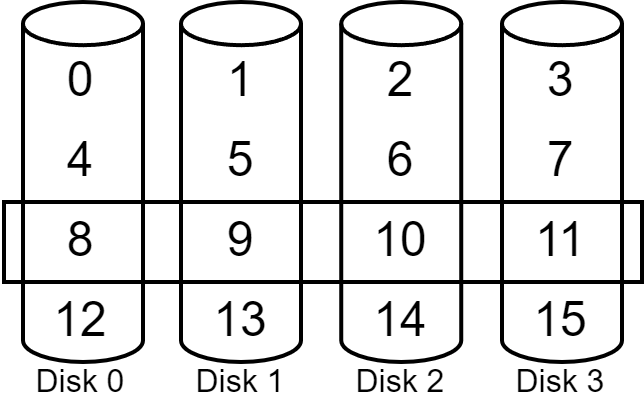
\includegraphics[width=0.3\linewidth]{images/strip.png}
    \caption{Data striping}
\end{figure}
Sequential accesses are evenly distributed across all drives, while random accesses occur naturally across all drives as well. 
Access to specific data blocks can be determined by computing the disk number and the offset:
\[\text{Disk}=\text{logical block number} \% \text{number of disks}\]
\[\text{Offset}=\dfrac{\text{logical block number}}{\text{number of disks}}\]
Chunk size influences array performance: smaller chunks lead to increased parallelism, while larger chunks result in reduced seek times.
\renewcommand*{\arraystretch}{2}
\begin{table}[H]
    \centering
    \begin{tabular}{|cc|}
    \hline
    \textbf{Capacity}                    & $N$                                                 \\ \hline
    \textbf{Reliability}                 & $0$                                                 \\ \hline
    \textbf{Sequential reads and writes} & $N\cdot S \qquad N\cdot S$                          \\ \hline
    \textbf{Random reads and writes}     & $N\cdot R \qquad N\cdot R$                          \\ \hline
    \textbf{Mean Time To Failure}        & $\text{MTTF}_{\text{RAID }0}=\frac{\text{MTTF}}{N}$ \\ \hline
    \end{tabular}
    \caption{RAID 0}
\end{table}

\subsection{RAID 1}
RAID 1 is a data storage configuration where data is mirrored to a second disk. 
This provides high reliability, as the second copy can be used if a disk fails. 
However, writes are slower than on standard disks due to duplication, and using half of the capacity results in higher costs.

RAID 1 can theoretically mirror content over more than one disk, enhancing resiliency even if multiple disks fail. 
Additionally, with a voting mechanism, it can identify errors not reported by the disk controller. 
However, this is rarely used due to high overhead and costs.

\paragraph*{Mirroring}
Mirroring involves making two copies of all data, providing redundancy so that if one copy is lost or corrupted, the other can be used to recover the data.
This approach offers both high performance and data protection.
\begin{table}[H]
    \centering
    \begin{tabular}{|cc|}
    \hline
    \textbf{Capacity}                    & $\frac{N}{2}$                                                          \\ \hline
    \textbf{Reliability}                 & $\frac{N}{2}$                                                          \\ \hline
    \textbf{Sequential reads and writes} & $\frac{N}{2}\cdot S \qquad \frac{N}{2}\cdot S$                         \\ \hline
    \textbf{Random reads and writes}     & $N\cdot R \qquad \frac{N}{2}\cdot R$                                   \\ \hline
    \textbf{Mean Time To Failure}        & $\text{MTTF}_{\text{RAID }1}=\frac{\text{MTTF}^2}{2\cdot \text{MTTR}}$ \\ \hline
    \end{tabular}
    \caption{RAID 1}
\end{table}

\subsection{RAID 01}
RAID 01 is a RAID configuration where data is first striped across multiple drives using RAID 0 and then mirrored using RAID 1.
This provides both high performance and data redundancy. 
In the event of a failure in the RAID 0 stripe, the data remains available on the other drives, and the RAID 1 mirror provides an additional copy for protection. 
The minimum number of drives required for this configuration is four.

\subsection{RAID 10}
RAID 10 combines the mirroring of RAID 1 with the striping of RAID 0, offering both data redundancy and improved performance. 
In a RAID 10 setup, data is first mirrored across two or more drives (RAID 1) and then the mirrored data is striped across additional drives (RAID 0). 
This configuration provides high reliability and performance for both read and write operations, making it ideal for databases and other applications with high input output demands. 
RAID 10 requires a minimum of four drives.
\paragraph*{RAID 10 and RAID 01}
Both RAID 10 and RAID 01 offer the same performance and storage capacity. 
The critical difference lies in their fault tolerance: RAID 10 is more fault-tolerant than RAID 01. 
In RAID 10, the system can sustain multiple disk failures as long as no mirror pair loses all its drives.
In contrast, RAID 01 has a higher risk of total data loss if a disk failure occurs within the striped sets.

\subsection{RAID 4}
In RAID 4, one disk in the array stores parity information for the other $N-1$ disks. 
The parity bit is computed using the XOR operation.

\paragraph*{Writes}
There are two methods for updating parity during writes:
\begin{itemize}
    \item \textit{Additive parity}: calculates the new parity value by XORing all the recomputed block parity values with the new data value.
    \item \textit{Subtractive parity}: calculates the new parity value by XORing the old parity value with the new data value.
\end{itemize}

\paragraph*{Reads}
Reads in RAID 4 are efficient because data is evenly distributed across all non-parity disks. 
This ensures parallel read operations without significant performance degradation.
RAID 4 performs well with sequential reads and writes, leveraging parallelization across non-parity blocks. 
However, all writes on the same stripe update the parity drive once.

\paragraph*{Random writes}
Random writes can cause a bottleneck in RAID 4 due to the need to update the parity drive, potentially causing serialization.
 Writing to a RAID 4 array involves reading the target block and the parity block, calculating the new parity block, and then writing both the target and new parity blocks. 
This can degrade performance, especially if the parity drive is slow or has limited bandwidth.
\begin{table}[H]
    \centering
    \begin{tabular}{|cc|}
    \hline
    \textbf{Capacity}                    & $N-1$                                                                  \\ \hline
    \textbf{Reliability}                 & $1$                                                                    \\ \hline
    \textbf{Sequential reads and writes} & $(N-1)\cdot S \qquad (N-1)\cdot S$                                     \\ \hline
    \textbf{Random reads and writes}     & $(N-1)\cdot R \qquad \frac{R}{2}$                                      \\ \hline
    \textbf{Mean Time To Failure}        & $-$ \\ \hline
    \end{tabular}
    \caption{RAID 4}
\end{table}

\subsection{RAID 5}
In RAID 5, parity blocks are distributed evenly across all $N$ disks. 
Unlike RAID 4, writes are spread evenly across all drives. 
Random writes in RAID 5 involve:
\begin{enumerate}
    \item Reading the target block and the parity block.
    \item Calculating the new parity block by subtracting the old parity block from the target block.
    \item Writing the target block and the new parity block.
\end{enumerate}
This process involves four operations (two reads and two writes) distributed evenly across all drives.
\begin{table}[H]
    \centering
    \begin{tabular}{|cc|}
    \hline
    \textbf{Capacity}                    & $N-1$                                                                       \\ \hline
    \textbf{Reliability}                 & $1$                                                                         \\ \hline
    \textbf{Sequential reads and writes} & $(N-1)\cdot S \qquad (N-1)\cdot S$                                          \\ \hline
    \textbf{Random reads and writes}     & $N\cdot R \qquad \frac{N}{4}\cdot R$                                        \\ \hline
    \textbf{Mean Time To Failure}        & $\text{MTTF}_{\text{RAID }5}=\frac{\text{MTTF}^2}{N(N-1)\cdot \text{MTTR}}$ \\ \hline
    \end{tabular}
    \caption{RAID 5}
\end{table}

\subsection{RAID 6}
RAID 6 provides more fault tolerance than RAID 5, allowing for the concurrent failure of two disks. 
RAID 6 uses Solomon-Reeds codes with two redundancy schemes (P+Q), distributing parity blocks across all disks. 
This configuration requires a minimum of four data disks and two parity disks, resulting in six disk accesses for each write operation. 
The MTTF is calculated as:
\[\text{MTTF}_{\text{RAID }6}=\frac{2\cdot\text{MTTF}^3}{N(N-1)(N-2)\cdot \text{MTTR}^2}\]

\subsection{Comparison}
\begin{table}[H]
    \centering
    \begin{tabular}{|c|ccccc|}
    \hline
    \textbf{RAID} & \textbf{Capacity} & \textbf{Reliability} & \makecell{\textbf{Read write} \\\textbf{performance}} & \makecell{\textbf{Rebuild} \\\textbf{performance}} & \textbf{Applications}                 \\ \hline
    \textit{0}    & $100\%$           & N/A                  & Very good                       & Good                         & Non critical data                     \\
    \textit{1}    & $50\%$            & Excellent            & Very good, good                 & Good                         & Critical information                  \\
    \textit{5}    & $\dfrac{\left(N-1\right)}{N}$   & Good                 & Good, fair                      & Poor                         & Database                              \\
    \textit{6}    & $\dfrac{\left(N-2\right)}{N}$   & Excellent            & Very good, poor                 & Poor                         & Critical information                  \\
    \textit{01}   & $50\%$            & Excellent            & Very good, good                 & Good                         & \makecell{Critical information \\ with performance} \\ \hline
    \end{tabular}
\end{table}
\renewcommand*{\arraystretch}{1}

\paragraph*{Hot spares}
Many RAID systems include a hot spare, an idle, unused disk installed in the system. 
In the event of a drive failure, the array is immediately rebuilt using the hot spare, minimizing downtime.

\paragraph*{Implementation}
RAID can be implemented in either hardware or software.

Hardware RAID uses specialized controllers built into the motherboard or a separate expansion card, offering faster and more reliable performance by offloading RAID management to dedicated hardware. 
However, migrating a hardware RAID array to a different controller can be challenging.

Software RAID uses software drivers running on the computer's CPU. 
It is simpler to migrate and cheaper than hardware RAID, but it generally has lower performance and reliability due to the consistent update problem, which can occur if the CPU is not powerful enough or is occupied with other processes.